
%% For double-blind review submission, w/o CCS and ACM Reference (max submission space)


\documentclass[sigplan,10pt,review,anonymous, nonacm]{acmart}
\settopmatter{printfolios=true,printccs=false,printacmref=false}
%\settopmatter{printacmref=false, printfolios=false}
%% For double-blind review submission, w/ CCS and ACM Reference
%\documentclass[sigplan,review,anonymous]{acmart}\settopmatter{printfolios=true}
%% For single-blind review submission, w/o CCS and ACM Reference (max submission space)
%\documentclass[sigplan,review]{acmart}\settopmatter{printfolios=true,printccs=false,printacmref=false}
%% For single-blind review submission, w/ CCS and ACM Reference
%\documentclass[sigplan,review]{acmart}\settopmatter{printfolios=true}
%% For final camera-ready submission, w/ required CCS and ACM Reference
%\documentclass[sigplan]{acmart}\settopmatter{}

\setcopyright{none}
%%
%% This is file `sample-sigconf.tex',
%% generated with the docstrip utility.
%%
%% The original source files were:
%%
%% samples.dtx  (with options: `sigconf')
%% 
%% IMPORTANT NOTICE:
%% 
%% For the copyright see the source file.
%% 
%% Any modified versions of this file must be renamed
%% with new filenames distinct from sample-sigconf.tex.
%% 
%% For distribution of the original source see the terms
%% for copying and modification in the file samples.dtx.
%% 
%% This generated file may be distributed as long as the
%% original source files, as listed above, are part of the
%% same distribution. (The sources need not necessarily be
%% in the same archive or directory.)
%%
%% Commands for TeXCount
%TC:macro \cite [option:text,text]
%TC:macro \citep [option:text,text]
%TC:macro \citet [option:text,text]
%TC:envir table 0 1
%TC:envir table* 0 1
%TC:envir tabular [ignore] word
%TC:envir displaymath 0 word
%TC:envir math 0 word
%TC:envir comment 0 0
%%
%%
%% The first command in your LaTeX source must be the \documentclass command.
%\documentclass[sigconf]{acmart}

\usepackage[english]{babel}
\usepackage{blindtext}
\usepackage{multirow}
\usepackage{CJKutf8}

\usepackage{booktabs}
\usepackage{subfigure}
\usepackage{xspace}
%%\usepackage{amsmath}
\usepackage{epstopdf} 
\usepackage{algorithm}
\usepackage{url}
%%\usepackage{algorithmicx} 
\usepackage{algpseudocode}
%%\usepackage{color}
\usepackage{ulem}

\newcommand{\btree} {B+tree\xspace}
\newcommand{\txtree}{STM-based GPU \btree\xspace}
\newcommand{\base}{STM-based GPU B+tree\xspace}
\newcommand{\baseshort}{STM GB-tree\xspace}
\newcommand{\locktree}{lock-baed GB-tree\xspace}
\newcommand{\ucdavis}{lock-based GPU B-tree\xspace}
\newcommand{\ucdavisshort}{Lock GB-tree\xspace}
\newcommand{\sys} {uniRDMA\xspace}
\newcommand{\native} {bare-metal RDMA\xspace}

%% NOTE that a single column version may be required for 
%% submission and peer review. This can be done by changing
%% the \doucmentclass[...]{acmart} in this template to 
%% \documentclass[manuscript,screen]{acmart}
%% 
%% To ensure 100% compatibility, please check the white list of
%% approved LaTeX packages to be used with the Master Article Template at
%% https://www.acm.org/publications/taps/whitelist-of-latex-packages 
%% before creating your document. The white list page provides 
%% information on how to submit additional LaTeX packages for 
%% review and adoption.
%% Fonts used in the template cannot be substituted; margin 
%% adjustments are not allowed.
%%
%%
%% \BibTeX command to typeset BibTeX logo in the docs
\AtBeginDocument{%
  \providecommand\BibTeX{{%
    \normalfont B\kern-0.5em{\scshape i\kern-0.25em b}\kern-0.8em\TeX}}}

%% Rights management information.  This information is sent to you
%% when you complete the rights form.  These commands have SAMPLE
%% values in them; it is your responsibility as an author to replace
%% the commands and values with those provided to you when you
%% complete the rights form.
%\setcopyright{acmcopyright}
%\copyrightyear{2018}
%\acmYear{2018}
%\acmDOI{XXXXXXX.XXXXXXX}



%%% These commands are for a PROCEEDINGS abstract or paper.
%\acmConference[Conference acronym 'XX]{Make sure to enter the correct
%  conference title from your rights confirmation emai}{June 03--05,
%  2018}{Woodstock, NY}
%%
%%  Uncomment \acmBooktitle if th title of the proceedings is different
%%  from ``Proceedings of ...''!
%%
%%\acmBooktitle{Woodstock '18: ACM Symposium on Neural Gaze Detection,
%%  June 03--05, 2018, Woodstock, NY} 
%\acmPrice{15.00}
%\acmISBN{978-1-4503-XXXX-X/18/06}


%%
%% Submission ID.
%% Use this when submitting an article to a sponsored event. You'll
%% receive a unique submission ID from the organizers
%% of the event, and this ID should be used as the parameter to this command.
%%\acmSubmissionID{123-A56-BU3}

%%
%% For managing citations, it is recommended to use bibliography
%% files in BibTeX format.
%%
%% You can then either use BibTeX with the ACM-Reference-Format style,
%% or BibLaTeX with the acmnumeric or acmauthoryear sytles, that include
%% support for advanced citation of software artefact from the
%% biblatex-software package, also separately available on CTAN.
%%
%% Look at the sample-*-biblatex.tex files for templates showcasing
%% the biblatex styles.
%%

%%
%% The majority of ACM publications use numbered citations and
%% references.  The command \citestyle{authoryear} switches to the
%% "author year" style.
%%
%% If you are preparing content for an event
%% sponsored by ACM SIGGRAPH, you must use the "author year" style of
%% citations and references.
%% Uncommenting
%% the next command will enable that style.
%%\citestyle{acmauthoryear}

%%
%% end of the preamble, start of the body of the document source.
\begin{document}

%%
%% The "title" command has an optional parameter,
%% allowing the author to define a "short title" to be used in page headers.
\title{\sys: Unified Virtual RDMA for Hybrid Virtual Environments}


%\author{Anonymous authors}
%\affiliation{%
%	\institution{Paper under double-blind review}
%	\city{}
%	\country{}
%}
%\email{}
%%
%% The "author" command and its associated commands are used to define
%% the authors and their affiliations.
%% Of note is the shared affiliation of the first two authors, and the
%% "authornote" and "authornotemark" commands
%% used to denote shared contribution to the research.


%%
%% By default, the full list of authors will be used in the page
%% headers. Often, this list is too long, and will overlap
%% other information printed in the page headers. This command allows
%% the author to define a more concise list
%% of authors' names for this purpose.
%-----------------\renewcommand{\shortauthors}{Anonymous Author, et al.}




%%
%% The abstract is a short summary of the work to be presented in the
%% article.
\begin{abstract}
RDMA network is gaining its popularity for high performance communication of distributed applications in datacenters. With virtualization becomes the de-facto layer of datacenters, RDMA network also needs to be virtualized. It is common for the datacenter to have virtual machine~(VM), container and sometimes container-in-virtual-machine as its basic resource provisioning entity. However, RDMA is virtualized in different ways for VMs and containers. And there is no coordination between the two resource users. To solve this problem, we present \sys~(unified virtual RDMA), which is a unified RDMA virtualization framework for both VMs and containers. In \sys, vRNICs (virtual RDMA network interface cards) are virtualized in host user-space, the URN core manages the vRNIC backends,  virtual RDMA network and hardware resources, and the management center issues the control plane or data plane policies. In our evaluation, \sys can be deployed in hybrid virtual environments within 5\% overhead to native RDMA.
\end{abstract}

%%
%% The code below is generated by the tool at http://dl.acm.org/ccs.cfm.
%% Please copy and paste the code instead of the example below.
%%
%\begin{CCSXML}
%<ccs2012>
% <concept>
%  <concept_id>10010520.10010553.10010562</concept_id>
%  <concept_desc>Computer systems organization~Embedded systems</concept_desc>
%  <concept_significance>500</concept_significance>
% </concept>
% <concept>
%  <concept_id>10010520.10010575.10010755</concept_id>
%  <concept_desc>Computer systems organization~Redundancy</concept_desc>
%  <concept_significance>300</concept_significance>
% </concept>
% <concept>
%  <concept_id>10010520.10010553.10010554</concept_id>
%  <concept_desc>Computer systems organization~Robotics</concept_desc>
%  <concept_significance>100</concept_significance>
% </concept>
% <concept>
%  <concept_id>10003033.10003083.10003095</concept_id>
%  <concept_desc>Networks~Network reliability</concept_desc>
%  <concept_significance>100</concept_significance>
% </concept>
%</ccs2012>
%\end{CCSXML}
%
%\ccsdesc[500]{Computer systems organization~Embedded systems}
%\ccsdesc[300]{Computer systems organization~Redundancy}
%\ccsdesc{Computer systems organization~Robotics}
%\ccsdesc[100]{Networks~Network reliability}

%%
%% Keywords. The author(s) should pick words that accurately describe
%% the work being presented. Separate the keywords with commas.
\keywords{RDMA, virtualization, virtual machine, contianer}

%% A "teaser" image appears between the author and affiliation
%% information and the body of the document, and typically spans the
%% page.

%%
%% This command processes the author and affiliation and title
%% information and builds the first part of the formatted document.


\maketitle




\section{Introduction}
RDMA(remote direct memory access), is a new type of high-performance network technology. RDMA is currently widely used in artificial intelligence, data processing, and high-performance computing. For examples, TensorFlow, Spark, and Hadoop [21] all have supported RDMA. With hardware protocol stack and zero copy technologies, RNICs(physical RDMA network cards) can bypass the kernel to read/write remote memory data according to the work requests of applications, without the participation of remote CPU. Therefore, RDMA has high throughput, low latency and low CPU load.

The core technology of cloud computing is virtualization, mainly including container and virtual machine. The container is a lightweight isolated runtime environment, does not need device emulation, and has low performance loss. The virtual machine has strong isolation and is more secure, but the performance loss is large. Both virtual machines and containers have been widely used, and the trend has become the unified deployment and management for hybrid virtual environments. For example, VMware's virtualization platform vSphere and ReadHat's container cloud platform OpenShift, both clearly support the unified deployment and management of virtual machines and containers in the latest version.

RDMA virtualization is necessary for cloud applications to exploit RDMA. RDMA virtualization not only needs to maintain high performance and manageability, but also have generality for hybrid virtual environments. Therefore, our RDMA virtualization goals are as follows:

\begin{itemize}
\item {\verb|Generality|}: To form unified RDMA virtualization, single centralized virtual layer should be set up, which is provided to virtual machines and containers with general interfaces.
\item {\verb|High performance|}: Virtual RDMA should be close to native RDMA in terms of throughput, latency, and CPU load. Meanwhile it should be suit for large-scale virtual cluster.
\item {\verb|High manageability|}: In RDMA virtualization, container and virtual machine characteristics should be maintained to realize portability, isolation and network management.
\end{itemize}

RDMA has different hardware characteristics and working mechanisms compared to traditional network. Therefore, RDMA virtualization is different from traditional network virtualization. Current RDMA virtualization work mainly includes hardware virtualization and software virtualization. However, none of the existing solutions can meet all above goals.

The representative of hardware virtualization is SR-IOV. Its virtual layer is located in the hardware. Although the isolation and high performance are maintained,  SR-IOV lacks portability and other manageability without software virtual layer. In software virtualization, existing solutions treat virtual machines and containers differently. For containers, FreeFlowl~\cite{kim2019freeflow} forwards all RDMA commands to the virtual layer, and that is ineffective because of losing RDMA's kernel by-pass. For virtual machines, HyV avoids forwarding overhead by mapping RDMA resources, but lacks the management of virtual RDMA networks; although MasQ makes up for this problem, its virtual layer is located in kernel space. Extending MasQ to the container environment will lose lightweight  management in user space for containers.

We proposes an unified RDMA virtualization framework for both containers and virtual machines, namely uniRDMA, which achieves high performance and high manageability. UniRDMA is mainly composed of single centralized uniRDMA virtual layer and general uniVerbs interfaces. All managements are concentrated in the user space virtual layer; the UniVerbs interface is general to the RDMA applications in virtual machines or containers.

There are mainly two challenges in the design of uniRDMA: First, virtual machines and containers are essentially different virtualization technologies. Virtual machines are under the management of hypervisor in kernel space, containers are isolted runtime mainly about user space. It is a challenge to build a centralized virtual layer for both containers and virtual machines; second, mapping all RDMA resources is the key idea to achive high performance. However, the existing solutions only implement the mapping operation in the same process for virtual machine. In this paper, the virtual layer belongs to another host process. So, it is also another challenge to map all RDMA resources.

To address the first challenge, uniRDMA separates the control and use of RDMA resources in virtulization, builds multiple vRNICs in single unified user space virtualization layer. Each vRNIC encapsulates virtual RDMA resources, and isolates with others by hardware virtualization. Moreover, through a common file-based shared memory queue, each vRNIC has a general interface for virtual machines and containers. For the second challenge,  at first, virtual RDMA resources in vRNICs are mapped to physical RNICs, and then shared memory are used to ensure RDMA resources in applications are mapped to vRNICs in the virtual layer.

We implements the prototype of uniRDMA and evaluate uniRDMA against with hardware virtualization, software virtualization FreeFlow, and native RDMA in different benchmarks, such as throughput, latency, scalability, and real-word applications. From the result, uniRDMA's performance is close to native RDMA in both virtual machine and container environments, and is significantly better than FreeFlow. The throughput can reach up to 6 times that of FreeFlow, and the latency can reach down to 40\% of FreeFlow.uniRDMA also has high scalability and adapts to real-world RDMA applications in hybrid cloud environments.

The main contributions in this paper are as follows:

(1)Unified RDMA virtulization in hybrid virtual environments is firstly proposed in this paper and uniRDMA is general RDMA virtualization framework,  while maintaining high performance and high manageability.

(2)uniRDMA are evaluated and the results proved that uniRDMA maintains high performance close to native RDMA.


\section{Background}
In this section, we first introduce the brief background, including virtualization and RDMA. 

\subsection{Cloud and Virtualization}
Cloud is popular for its efficiency and elasticity, and virtualization is the basic for clouds. Nowadays, VMs and containers are both common virtual instances in clouds. VMs need emulate whole virtual hardware environments for guest operation system with hypervisor (kernel-space). So, applications in VMs is isolated by guest OS with more security but higher overhead. Containers are shared with the host OS but with run-time isolation. So, containers have low overhead and fast boot-up time.

For software virtualization of I/O devices, there are two main choices for where to emulate the device: kernel-space and user-space. In kernel-space, the codes of device emulation are inserted into hypervisor or host kernel. Compared to kernel-space, there are three advantages for user-space: first, the attack surface is limited for user-space with minimal inserted code into kernel/hypervisor; second, management development is flexible in user-space; third, the inserted codes are often dependent on hardware-specific APIs (e.g. OS architecture, device driver). For example, vhost-net~\cite{vhost-net} is the kernel-space network device and vhost-user-net~\cite{vhost-user-net} has user-mode virtual device. 

\begin{figure}[!ht]
\centering
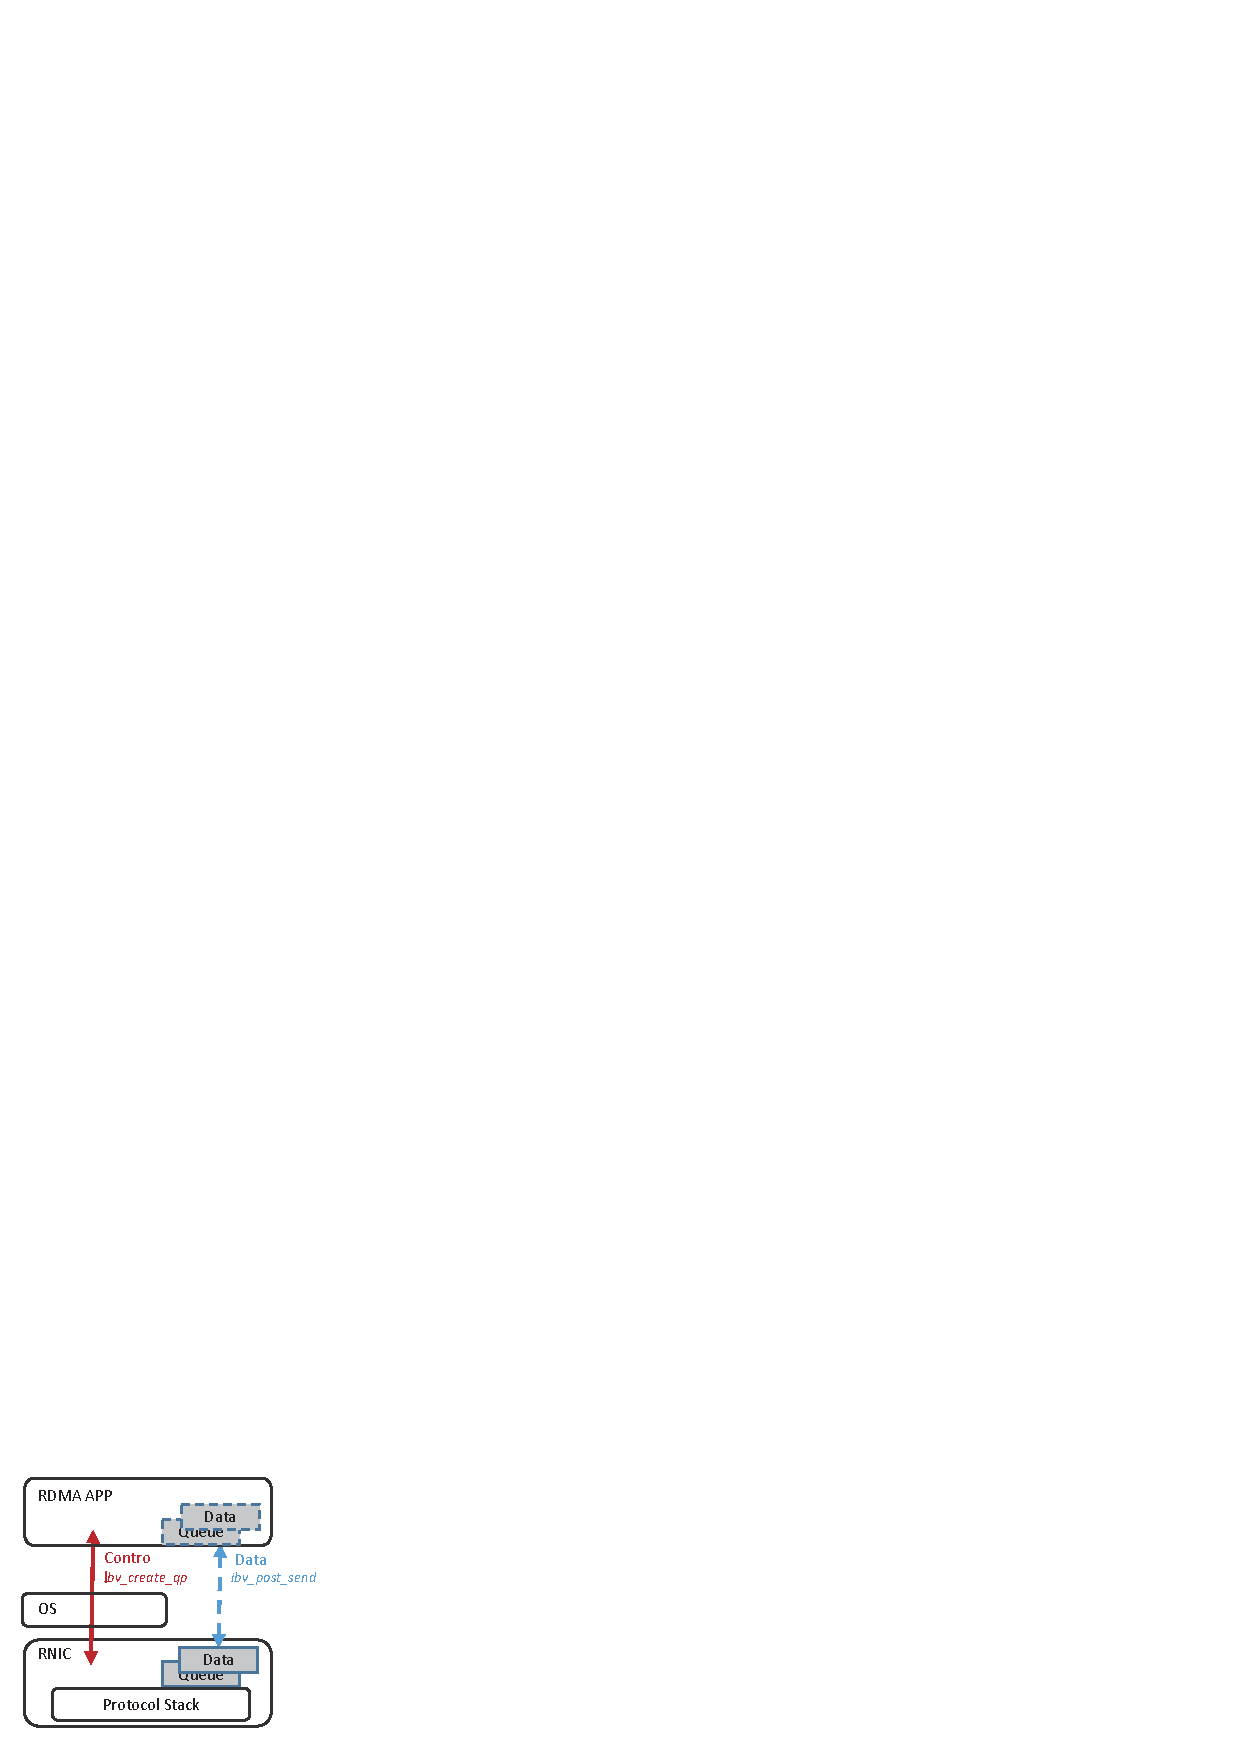
\includegraphics[width=0.8\linewidth]{images/rdma-feat.png}
\caption{Host RDMA Architecture: the control path and data path are separated}
\label{fig:rdma-feat}
\end{figure}

\subsection{RDMA}
As popular high-performance network in supercomputing, RDMA has hardware protocol stack and zero copy technology. With RDMA, applications can bypass the kernel to read and write remote memory data, without the participation of remote CPU. 

Verbs~\cite{verbs} is the basic interface for applications to utilize RDMA. It is similar as socket for traditional network applications. As shown in Figure~\ref{fig:rdma-feat}, RDMA Verbs is separate to control path and data path to achieve high-performance. In control path: applications open device and setup the RDMA context. The main resources in RDMA context include Queue Pairs (QPs), Complete Queues(CQs), Memory Regions (MRs). The control verbs include ibv\_create\_qp, reg\_mr;  In data path: applications directly use RDMA resources to transport data and the transport is asynchronous. In specific, applications fillwith the work request into the Send Queue or Receive Queue in a QP, each work request includes the address, size and key of the message. Then the RNIC can execute the operation. The data verbs include ibv\_post\_send and ibv\_post\_recv. Compared control path, data path bypasses the kernel to avoid context switch.

In a RDMA workflow, the communication is based on Queue Pair (QP). The application writes the RDMA work request to the QP, and then ``press''  the RNIC's doorbell register, which is mapped to application when context init, and the RNIC's hardware processor will execute the work request in the QP to forward data. There are two modes for RDMA connect-based communication: one-sided and two-sided. One-sided is that remote server is awareness when client reads or writes its registered memory; Two-sided is that one sends messages after the peer is ready to receive.

%%\section{Overview}
The architecture of uniRDMA is shown in Figure~\ref{fig:framework-overview}. uniRDMA consists of three parts: Verbs libraries in guest, vRNIC (frontend and backend) and management center.

(1) The verbs libraies in guests: They are modified to achive transparency for applications. In specific, we forward the verbs command to uniRDMA frontend. Thus, applications in guest can use verbs libraries same as native RDMA.

(2) vRNIC frontend and backend: Control and data path are separate to achive high-performance. In control path, the vRNIC frontend forwards RDMA verbs to backend in uniRDMA virtual layer, and vRNIC backend execute them; In data path, vRNIC frontend directly use the mapped RDMA resources (e.g. QPs or MRs). The resources are mapped to backend by shared memory.

(3) Management center: To make a centralized management, a management center connect with each host's uniRDMA backend. For example, center configures each vRNIC address, define routing rules and maitain the mapping for vRNIC connections.

\begin{figure}[!ht]
	\centering
	\includegraphics[width=1\linewidth]{images/framework-overview.png}
	\caption{uniRDMA Framework Overview}
	\label{fig:framework-overview}
\end{figure}
% 第4章 设计
\section{Design}

% URN的目标是实现一个统一的软件虚拟化架构,能够同时为虚拟机和容器提供RDMA服务,并实现对虚拟RDMA的统一管理。此外,该框架还需具备与原生RDMA接近的高性能。在本章,介绍了URN中的一些关键性设计工作。
The goal of URN is to provide a unified RDMA virtualization framework for the cloud environment where containers, virtual machines and containers inside virtual machine could coexist, even on the same server. In this framework, virtual and physical RDMA resources on one server are solely managed and scheduled by the URN core. The second design goal of URN is that the performance of virtualized RDMA should be close to the native RDMA. The third design goal is to be transparent to the vanilla RDMA applications, and to bring minimal code changes to RDMA software stack. In this section, we introduce some key design details.

\subsection{vRNIC Design}

% vRNIC是一个软件的虚拟RDMA设备,包含前后端,前端负责为上层verb库提供接口并转发RDMA 命令,后端在主机端,通过与URN core或verbs库交互,以模拟guest对vRNIC的RDMA操作。 我们继承了控制和数据通道分离的哲学,和已有的RDMA虚拟化方案一样,如hyv和MasQ,控制路径上guest应用在本地的虚假RDMA上下文中执行verbs命令,并经过FE转发到BE维持的真实RDMA上下文中执行,之后将结果返回给guest;在数据路径上,将guest应用的RDMA资源与vRNIC BE上下文中的RDMA资源进行映射,guest应用的RDMA资源被注册到了物理网卡中,之后guest应用可以在本地直接使用RDMA资源进行数据操作。
vRNIC is a virtual device, which consists of the frontend and backend. The frontend forward the commands of Verbs library in the guest user space to backend. The backend execute the commands by interacting with the physical RNIC through Verbs library in host user space. We inherited the philosophy that the control path and data path of RDMA operations are virtualized in different ways\cite{pfefferle2015hybrid}\cite{he2020masq}\cite{kim2019freeflow}. On the control path, para-virtualization technique is used that control commands from the guest Verb library are served by the frontend and forwarded to backend. On the data path, direct-passthrough technique is used that applications in the guest environment can directly map and use physical RDMA resources so that no guest OS kernel or host virtualization layer is involved when sending and receiving network pakages. The details of memory mapping implementations in URN framework is described in section 5 Implexxx.

% 前端:
% vRNIC前端作为vRNIC的设备接口提供给guest中的verbs库。Verbs命令可以通过前端转发到后端。在虚拟机中,vRNIC前端位于guest内核空间,并模拟原生的RDMA内核驱动为上层的verbs库提供与原生一致的接口,例如设备总线,设备文件。因此,当虚拟机中的前端加载后,可以直接使用未修改的verbs库。这样的好处是让URN系统更加稳定。
%The vRNIC frontend acts as the device interface of the vRNIC for Verbs library in the guest environments. The Verbs commands can be forwarded from the frontend to the backend. 
The design of the vRNIC frontend is different in containers and VMs. In VMs, the frontend is located in the guest kernel space, and it exposes the interface of native RDMA kernel driver to Verbs library, in the form of device class and device file. Thus, unmodified Verbs library can be used in VMs and this makes URN framework transparent to the evolution of Verbs library in the virtual machine.
% 然而,在容器中,无法像虚拟机一样提供对verbs用户库透明的接口。这是因为,如果前端位于主机内核空间,并提供与原生RDMA内核驱动一致的虚拟设备接口给verbs用户库。这些虚拟设备接口将与原生的物理设备接口一同暴露给verbs用户库. verbs用户库在未经修改的前提下, 无法区分使用的接口是前端提供的还是RDMA内核驱动提供的。
However,in containers, it is impossible to provide the unmodified interface for Verbs library. Because, if the frontend in host kernel space provides the same interfaces same as RDMA kernel driver. Note that both the virtual device interfaces and physical device interfaces are exposed to Verbs library in containers, and Verbs cannot distinguish them without extra modification in containers.  
% 因此,我们直接将前端实现在用户空间,作为一个用户库提供,并链接到Vers库。特别的,Verbs库中与设备接口相关的系统调用被替换为与前端交互的函数调用。容器应用程序在链接这个前端库后便可以转发verbs命令到后端。
%因此,容器前端的另一个好处是与Verbs交互完全在用户空间,没有系统调用开销。最后,注意虚拟机和容器的前端都是设备无关的,因为它们仅仅与通用的Verbs库及后端交互。
Thus, the frontend for containers is in user space, provided as a costumed library, and linked to Verbs library. In specific, in Verbs library, the origin device interface are replaced with the function call to the frontend. The Verbs commands can be forwarded to vRNIC backends after loading the frontend library. 
Thus, another advantage is that the interact with upper Verbs library is wholly finished in user space without the overhead of system calls. Finally, note that all frontends is hardware-independent because they only interact with the hardware-independent Verbs library and backends.


% 后端:后端在哪,为什么用户空间?
% 在URN中,vRNIC 后端实现在主机的用户空间作为一个虚拟设备。在用户空间主要有三方面的优势:1y用户空间更适合管理:开发管理功能,在用户空间更加简单并且灵活;2,用户空间的稳定性更好:由于用户空间不存在面向内核的攻击面;3,用户空间的兼容性更好,因为用户空间对于不同的系统架构、内核版本和设备内核驱动兼容.
 In URN, the vRNIC backend locates in the host user space as a virtual device. There are three advantages for vRNIC backend in user space: first, user space is more suitable for management: the develop of management functions is easier and more flexible in user space; second, user space provides higher stability: the attack surface for kernel is not in user-space; third, the user space provides higher compatibility because it is often independent on specific APIs (e.g. system architecture, kernel version and device kernel driver).

% 后端中需要维持哪些内容,为什么要维护?
% 后端作为虚拟设备,为guest提供的RDMA服务最终仍然需要由通过使用物理RNIC来完成。因此,在后端中,需要维护三方面的信息:1, 来自guest的虚拟的RDMA上下文信息: 该信息在接受前端请求时便可以记录下来,例如guest中应用的MR的虚拟地址GVA;2,主机中的真实RDMA上下文信息:这些信息直接通过verbs库来维持,并且能被物理网卡设备识别;3,两者的映射关系。在解析前端命令并调用Verbs库后,进行指定。基于上述信息,后端可以通过与UNR core进行交互,来实现对虚拟RDMA网络的管理以及对vRNIC使用硬件资源的统一管控。关于管理功能主要在URN core章节介绍。
As a virtual device, the RDMA service provided by the backend should be executed through the physical RNIC. Thus, there are three aspects of information need to be maintained: 
a) attributes for the virtual RDMA contexts in the guest environment: they can be recorded when the commands are received from the frontend in the guest, e.g. the GVA (guest virtual address) of MR in the application inside the guest.
b) attributes for the physical RDMA contexts in the host: they is maintained through the Verbs library and can be recognized by physical RNIC, e.g. the HVA (Host Virtual Memory) of MR in the host.
c) the mappings between virtual and physical attributes: the mapping relationship are assigned when the Verbs commands from the frontend are executed. 
Based on the above information, the vRNIC backend can interact with the URN core to achieve the virtual RDMA network management and the hardware source management. And the management are mainly introduced in section xxx.

\begin{figure}[!ht]
	\centering
	\includegraphics[width=0.7\linewidth]{images/vrnic-backend.png}
	\caption{The information maintained in vRNIC backends}
	\label{fig:route-config}
\end{figure}

\subsection{Verbs and Hardware-specific Libraries}
% 1,根据vRNIC的设计,需要对verbs库及设备相关库进行必要的修改。对于原生RDMA来说,verbs库是设备无关的,提供通用的verbs接口给上层应用,并通过通用的设备接口与内核驱动进行交互。硬件相关的库主要隐藏了与RDMA资源的重要细节,例如,资源的内存分配,以及QP队列的填充操作等等。
According the design of vRNIC, there are some necessary modifications in Verbs library and hardware-specific library, e.g. libmlx4. For native RDMA, the Verbs library is hardware-independent, which provides general interface to upper applications and interact with RDMA kernel driver through the general device interface. The hardware-specific library mainly hides the key details about manipulating RDMA resources, such as allocating memory and fillwithing QP. 

%在URN中,Verbs库中的修改主要与接口有关,在设备相关库中,修改主要与内存映射操作以及地址翻译等相关。因为内存映射在应用的内存地址和网卡记录的地址之间带来了不一致的问题。首先,在主机端,我们在设备相关库中,修改了地址分配的函数,在修改后,可以直接指定映射后的地址去注册RDMA资源到物理网卡。
In URN, the modifications in Verbs library is mainly about interfaces; And the modifications in hardware-specific library is mainly memory mapping operations, and the resource memory address translation, because the memory mapping brings inconsistent ion between the applications' memory address and the RNIC's recorded registered address (in vRNIC backend address space).

Firstly, in host, we modified the memory allocation about RDMA resources in hardware-specific library. After modification, we can assign the mapped memory when registering RDMA resources (e.g. QPs) to physical RNIC.

% 对于容器来说,我们修改了RDMA内核驱动与verbs之间的接口,并且用到前端的接口进行替换。对于容器来说,不同修改verbs用户库因为前端在内核中模拟了同样的设备接口。对于虚拟机和容器来说,所有的地址翻译都是需要的。
For containers, we modified interface between Verbs library and RDMA kernel driver, and replace with the interface to vRNIC frontend. For VMs, we do not modify the Verbs library due to the simulated device interface is same as native RDMA. For both VMs and containers, the address translation is needed in data path.

\subsection{URN Core}
% URN core被设计用来管理虚拟RDMA网络和物理RDMA资源在每个主机上, 包括实例化vRNIC后端,虚拟网络配置和RDMA资源限制等。同样的,URN实现在用户空间。
URN core is designed to manage the virtual and physical RDMA resources for the host, including instantiating vRNIC backends, virtual network configuration and RDMA resources limitation. Also, URN is in host user space for the same reasons in section xxx.

% URN core如何实例化vRNIC后端?
%注意到后端在主机用户空间,因此,URN core有必要建立一个消息通道在vRNIC和所有guest之间,因为URN core(主机用户空间) 是隔离虚拟机监视器或容器的。当guest需要vRNIC时,他们可以请求URN core在主机用户空间中实例化相应的后端。为了构建这个通道,我们使用了UNIX套接字对于虚拟机及容器环境。当虚拟机或容器需要一个新的vRNIC时,对套接字发出的实例化请求会被URN处理。为了快速支持多个实例化请求,这个过程中采用了反应器模式。
Recall that the vRNIC backends is in host user space, it is necessary to build a communication channel between URN and all guests, because the URN core is another process in host and the isolated with both containers and the hypervisor(VMs). When guests need a vRNIC, they can request the URN core to instantiate corresponding backend in host user space. To build this channel, we utilize the UNIX socket for both VMs and containers. When VMs or containers need a new vRNIC, the instantiating request to socket are deal with URN. To support multiple request rapidly, the reactor mode are adopted in the process. 


% URN core 对BE提供统一接口?
% 除了实例化vRNIC后端,URN core 还包括了管理功能:包括虚拟网络管理和硬件资源管理。 为了实现这些管理,URN core 首先要监控vRNIC后端的属性和上下文,并在URN核心中汇总信息(如资源内存映射)。为此,URN提供了记录RDMA上下文及属性的接口。在RNIC后端中,这些记录接口在Verbs命令执行后被调用,以更新记录信息;
%其次,URN core还提供了控制接口,并且用户定义的配置或控制策略可以部署到vRNIC后端。记录和控制接口都是回调函数,当vRNIC后端实例化时,它们被注册到vRNIC后端。接下来介绍虚拟网络配置和硬件资源管理:
Besides instantiating vRNIC backends, the URN core is also designed for the management: including virtual network and hardware resources. To achieve the management, at first, the attributes and contexts in vRNIC backends should be monitored and the information (e.g. resource memory mapping) should be summarized in URN core. Thus, the URN provides the recording interfaces about the attributes and contexts, and the interfaces are executed in vRNIC backends when the Verbs commands are executed; 
second, the control interfaces are also provided and user-defined configuration or control policies can be deployed into vRNIC backends. Both recording and control interfaces are lots of callback functions and they are registered into vRNIC backends when vRNIC backends instantiating. Later, the virtual network configurations an hardware resources management are introduced:

% 具体讲URN core提供了哪些管理功能:
% 1, 虚拟网络构建:在云环境中,虚拟网络配置是实现很多功能的基础,例如多租户隔离、便携的虚拟机或容器迁移。虚拟网络配置包括了虚拟的网络地址,虚拟的路由规则以及其他软件定义的配置协议。URN在用户空间,支持灵活的虚拟RDMA网络配置。
In clouds, virtual network configuration is important for lots of features, such as multi-tenant isolation and portable guest migrations. The virtual network configuration includes virtual network address, virtual network routing rules and other software-defined information. URN support flexible virtual RDMA network configurations in user space. 
%首先,通过vRNIC后端控制接口,URN可以用vRNIC后端维护的虚拟地址(例如vGID)配置vRNIC,该地址可以通过vRNIC前端反映到客户端的应用程序中。
First, through the control interface to vRNIC backends, URN can configure the vRNIC with virtual address (e.g. vGID) which maintained in vRNIC backends, and the address can be reflected into applications in the guest through the vRNIC frontend.
%其次,可以在每个URN核心中定义虚拟RDMA网络路由规则。每个vRNIC后端都配置了组ID,路由规则定义为:{group ID1, group ID2, Policy}。一个关于查找路由规则的回调函数在实例化时注册到每个vRNIC后端。这样,路由规则就可以实时地反映到服务器的所有vRNIC后端中。例如,如图~\ref{fig:route-config}所示,容器1和容器2的vrnic被配置到同一组中,因此允许创建RDMA连接。作为对比,容器和虚拟机1是隔离的因为属于不同组。最后,vgid在物理RNIC中不能被识别,网络地址映射在vRNIC后端被创建和更新。如果路由规则允许,这对vgid将被转换成物理的gid来创建RDMA连接.
Second, the virtual RDMA network routing rules can be defined in each URN core. Each vRNIC backend is configured with the group ID and the routing rules can be defined as: {Group ID1, Group ID2, Policy}. A callback function about lookuping routing rules is registered to each vRNIC backends when instantiating vRNIC backends. Thus, the routing rules can be reflected in real time for all vRNIC backends in the server. For example, as shown in Figure~\ref{fig:route-config}, the vRNICs for container 1 and container 2 are configured into the same group, thus RDMA connections are allowed to create. In contrast, the container 1 and VM 1 are isolated RDMA network because different groups. Finally, the vGIDs is not recognized in physical RNIC, and the network address mappings are created and updated in the vRNIC backends. If the routing rules allow, the pair of vGIDs will be translate to physical GIDs to create the RDMA connection.

\begin{figure}[!ht]
	\centering
	\includegraphics[width=1.0\linewidth]{images/route-config}
	\caption{Group Configuration and Routing: The vRNICs of container 1 and container 2 are configured in one group. Thus, two containers can create RDMA connections. And VM 1 are not allowed to create RDMA connections to containers in this figure because it is not added into the group. }
	\label{fig:route-config}
\end{figure}


\begin{figure}[!ht]
	\centering
	\includegraphics[width=0.7\linewidth]{images/urn-interface.png}
	\caption{URN Core Interface: QP examples}
	\label{fig:framework-overview}
\end{figure}

% 2 对硬件资源的管理: 主要分为两部分,一对vRNIC使用的资源进行限制,以QP资源为例子;二,对硬件资源通过灵活映射的方式提高利用率, 以VF映射为例子。
% 硬件资源管理是URN core的另一个重要特性。在URN内核中,每个vRNIC使用的硬件资源都是受限的。例如,QP是RDMA的关键资源,创建过多的QP可能会降低RDMA的性能。URN核心还可以通过记录接口监视服务器中的所有QPs。另外,可以在URN core中定义QPs的最大值,也可以将熔断策略注册到vRNIC后端。当QPs对于vRNIC过多时,后续的creat_qp将被中止。
Hardware resource management is another important feature in URN core. In URN core, hardware resources can be limited for each vRNIC. For example, QP is the key resource in RDMA and many QPs may decrease the performance of RDMA. The URN core can monitoring all QPs in the server through the recording interface. The maximum of QPs can be defined in URN core and the fusing policy can be also registered to vRNIC backends. When QPs are excessive for a vRNIC, the subsequent creat\_qp will be aborted. 
% 此外,URN核心中可以灵活地利用硬件资源。在URN core中,所有硬件资源的状态信息都可以通过各个vRNIC后端或Verbs库进行汇总。通过灵活地将虚拟RDMA上下文映射到物理硬件资源上,可以实现硬件资源的高效利用。例如,VFs可用于云中的性能隔离。但是VFs是有限的,有最大值,如63~126,而且VFs的分配是静态的。因此,如果客户机数量大于服务器中的VFs,则无法满足每个客户机的性能隔离。为了解决这个问题,URN core可以灵活地将VFs映射到vRNIC,实现每个客户端的性能隔离。当URN core发现vRNIC处于空闲状态时,URN core便会释放该vRNIC的VF, 并将其分配给其他已经就绪的vRNIC。
Besides, hardware resources can be utilized flexible in URN core. In URN core, the status of all hardware resources can be summarized by the vRNIC backends and the Verbs library. By flexibly mapping virtual RDMA contexts to physical hardware resources, efficient utilization of hardware resources can be achieved. For example, the VFs can be used for performance isolation in clouds. But VFs is limited with maximum e.g. 63~126, and the allocation of VFs is static. Thus, if the guests is more than the VFs in a server, the performance isolation for each guest is not meet. To solve this problem, the URN core can flexibly map VFs to vRNICs to achieve the performance isolation for each guest. If the URN core finds that the vRNIC is idle, the VF of the vRNIC is released by URN core and it can be allocated to another ready vRNIC.


\subsection{Discussions}
% 4.4 discussion 
% (1)云环境管理: 云环境中需要更多的管理功能,例如QoS,流量计费等策略。显然,这些策略依赖RDMA中数据路径的信息,例如消息大小。然而,在URN中,vRNIC前端和后端都在数据路径中被绕过。因此,我们应该将这些管理扩展到guest中的特定硬件库中,因为数据路径是在这个库中实现的。对于策略,可以通过管理中心进行配置和分发。注意,这些扩展需要所有客户机都信任库,并且这些修改应该包含在TCB(可信计算库)中。
(1) More management for clouds: There are lots of important managements in clouds, e.g. QoS, metering and so on. Apparently, these policies are dependent on the information about data path in RDMA, e.g. the message size. However, in URN, both vRNIC Frontend and Backend are bypassed in the data path. Thus, we should extend these management into specific-hardware library in guest, because data path is mainly implemented in this library. The policies can be defined and distribute through the management center. Note that, these extension needs that the library is trusted for all guests, and the modification should be included into TCB (trusted computing base).


% (2)虚拟实例迁移:容器或虚拟机迁移在云中有很多好处,例如资源利用和故障转移。通过使用虚拟RDMA网络,URN可以支持脱机迁移,而无需为应用程序重新配置物理RDMA网络。具体来说,在重新启动迁移的虚拟实例后,应用程序可以通过相同的网络地址重建RDMA连接。唯一的工作是修改URN core中的地址映射.目前,由于RDMA应用程序中的内存区域在旁路或单侧通信下可能存在不确定性,因此对动态迁移仍然存在困难。该问题与URN无关.
(2) Virtual Instances Migration: Migration of containers or VMs has many benefits in clouds, e.g. resource utilization and fail-over. With the virtual RDMA network, URN can support offline migration without reconfiguring the physical RDMA network for applications. In specific, after rebooting the migrated virtual instance, the application can rebuild the RDMA connection through the same network address. The only work is modifying the address mapping in URN core. Currently, for live migrations, it is still hard because memory regions in RDMA application may be uncertain under bypassing or one-side communication. And the problem is unrelated to URN.

% (3) 其他网络扩展: RDMA也可以被用来加速其他网络应用,例如基于TCP/IP网络协议栈的socket应用。现有的工作包括vSocket和SockDirect等。在URN中,同样可以通过扩展已有架构来实现优化guest socket的效果。通过修改vRNIC的前后端,可以将guest的socket命令转发到后端由RDMA执行。对应的,还需要修改与容器中的socket用户库,以将命令直接通过前端转发到后端。在后端,将socket命令通过RDMA网络执行,然后返回给guest。对于数据路径,同样可以通过映射方式实现零拷贝。
(3) Other network extensions: RDMA can also be exploited to optimize the performance of other network applications,  such as TCP/IP.  Existing works include vSocket ~\cite{wang2019vsocket}, SockDirect~\cite{li2019socksdirect} so on. In URN, the socket applications in the guest can also be optimized through some extensions. By modifying the vRNIC frontend and backends, the socket commands can be forwarded to the backend and executed through physical RDMA network. For data paths, zero copy can also be achieved by mapping.

%\section{Implementation}
 We implement uniRDMA in Linux environments, the hypervisor of VM is KVM and the container engine is Docker. The whole implementaion is also
\section{Evaluation} \label{eval}
In this section, we evaluate the performance of \sys based on the RDMA test tools and real applications. We expect to answer the following questions:

\begin{itemize}
\item How about the performance of \sys compared to that of native RDMA for both VMs and containers?
\item Can \sys be adapted to the real-world RDMA applications in both VMs or containers?
\end{itemize}

\subsection{Experiment Methodology}
All experiments are carried out on two servers. The settings mainly include three parts: host server, container and virtual machine. 

Each host server is equipped with 4 Intel Xeon E7-4850 2.40GHz 16-core CPUs and 1 TB RAM. The RNIC used is Mellanox ConnectX-3 56 Gb/sec, which performs RDMA communication under Infiniband.  The operating system is CentOS 7.4.1708 (Linux 3.10.0-693.el7.x86\_64). The RDMA driver installed on the host server is Mellanox OFED 4.4-2.0.7.0~\cite{mlnx-ofed}. To keep the consistence, VMs and containers are built based on the same OS images as host. All virtual machines are based on QEMU(5.1.50)~\cite{qemu} enabled with KVM~\cite{kvm}. We provide 16 cores and 64 GB memory for each VM. We run containers using Docker(18.06.1-ce)~\cite{docker} and limit the CPU and memory resources to the same settings as the VM. In addition, all the applications are compiled with GCC/G++ 4.8.5 with the O3 compilation configuration. 


\subsection{Basic benchmark}
Throughput and latency are the key target of network performance. RDMA supports two different data transmission modes: one-sided and two-sided. Due to the difference performance between them, we evaluate them respectively.

Based on the RDMA benchmark test tool perftest~\cite{perftest}, we evaluated the throughput and latency of \sys, native RDMA, hardware virtualization SR-IOV, and software virtualization FreeFlow in virtual machines or containers. For two-sided operations (Send and Recv), we use the ``ib\_send\_bw'' and ``ib\_send\_lat'' commands; for one-sided operations (Write and Read), with Write as the representative, we use the ``ib\_write\_bw'' and ``ib\_write\_lat'' commands. The specific process is: after the RDMA connection is established between the client and the server, the bytes of transmitted message each time will be increased from 4B to 1MB, the data will be iteratively transmitted 1000 times with each message size, and finally the average throughput and latency are calculated.

(1) Throughput: The results of two-sided operation are shown in Figure~\ref{fig:send-bw}, and the one of one-sided operation are shown in Figure~\ref{fig:write-bw}. Whether \sys is in a virtual machine or in a container scenario, the throughput of its two-sided and one-sided operations is similar as SR-IOV and close to native RDMA.

Compared with FreeFlow, when the message is small, the throughput of \sys has reached 4-6 times that of FreeFlow. Because FreeFlow forwards all data commands to the software virtualization layer for processing. Therefore, the forward latency gradually accumulates and decrease the throughput significantly. However, \sys maps all RDMA resources to execute data commands in the user space of the container or virtual machine. Therefore, there is no latency for commands forwarding in data path.

\begin{figure}[!ht]
	\centering
	\includegraphics[width=1.0\linewidth]{images/send-bw.pdf}
	\caption{The Throughout of RDMA Send and Recv}
	\label{fig:send-bw}
\end{figure}

\begin{figure}[!ht]
	\centering
	\includegraphics[width=1.0\linewidth]{images/write-bw.pdf}
	\caption{The Throughout of RDMA Write}
	\label{fig:write-bw}
\end{figure}

When the message gradually increases, such as reaching 64KB, the throughput of each framework tends to be consistent. The reason is that the bandwidth is saturated, and the delay overhead of FreeFlow has been covered by waiting delay in RNIC.

(2) Latency: The results of two-sided operation are shown in Figure~\ref{fig:send-lat}, and the one of one-sided operation are shown in Figure~\ref{fig:write-lat}. Whether \sys is in a virtual machine or in a container scenario, the latency of its two-sided and one-sided operations is similar as SR-IOV and close to native RDMA.

Compared with FreeFlow, when the message is small, the latency of \sys has reached 40\%~60\% of FreeFlow because of FreeFlow's forwarding latency. Also, when the message gradually increases, such as reaching 64KB, the latency of each framework tends to be consistent. Because the main latency has been caused by RNIC data processing.

\begin{figure}[!ht]
	\centering
	\includegraphics[width=1.0\linewidth]{images/send-lat.pdf}
	\caption{The Latency of RDMA Send and Recv}
	\label{fig:send-lat}
\end{figure}

\begin{figure}[!ht]
	\centering
	\includegraphics[width=1.0\linewidth]{images/write-lat.pdf}
	\caption{The Latencty of RDMA Write}
	\label{fig:write-lat}
\end{figure}

\subsection{Real-world Applications}

The worth of RDMA is mainly about its optimized performance in real-world applications. RDMA virtualization needs to maintain the performance close to native RDMA. Therefore, we evaluate \sys and other frameworks in high-performance computing benchmark Graph-500. Graph-500 is a benchmark framework used to test the performance of the Message Passing Interface (MPI). Based on the constructed graph structure, users test the performance of breadth-first search (BFS) and single source shortest path (SSSP). The performance index is the number of edges traversed per second (traversed edges). per second, TEPS), the larger the value, the better the performance.

In this paper, the node scale of the computational graph in Graph-500 is set to 26, and the ratio of edges to points is set to the default parameter of 16. The constructed graph has a total of 2$^{25}$ vertices, with 2$^{29}$ edges, the entire graph occupies approximately around 16GB. When testing BFS and SSP, 16 MPI processes are scattered and executed on two nodes in turn, and the average value is taken according to the results of 12 tests. The data obtained is shown in Table Figure~\ref{fig:graph-500} (because there are core dump problems when using FreeFlow for Graph-500, the corresponding data is lacking).

As shown in Figure~\ref{fig:graph-500},  the performance of \sys is close to native RDMA. Because \sys bypasses the kernel and virtualization layer in the data path, and there is no forwarding latency.

\begin{figure}[!ht]
	\centering
	\includegraphics[width=1.0\linewidth]{images/graph-500.pdf}
	\caption{The Performance of Graph-500}
	\label{fig:graph-500}
\end{figure}
\section{Related Work}

% 对比已有工作与uniRDMA
\textbf{RDMA Virtualization}: The solutions of RDMA virtualization including hardware-based and software-based.

The basic solution is SR-IOV in hardware-based virtualization of RDMA. Its virtual layer is located in the hardware and are limited by hardware resources. In uniRDMA, the ioslation of SR-IOV are utilized and the unscable problems are soleved by dynamaic vRNIC mapping. 

In software virtualization, existing solutions donnot suit for hybrid virtual environments. FreeFlow's forward mechanism is different with uniRDMA. Its data path needs extra CPU to reduce the forward latency. Hyv and MasQ are not used in containers, but are similar with us because all have achieved zero-copy and by-pass by mapping all resources. Even though, the implemention of mapping are different at enssentional for two reasons: First, HyV and MasQ's mapping is in the same process and uniRDMA is inter-process; Second, HyV and MasQ's mapping management in kernel-space and our in user-space for more managablity and lightweight.


\section{Conclusion} \label{conclusion}
In this paper, we design a unified RDMA virtualization stack, namely \sys, which provides virtualized RDMA network for both VMs and containers on the same framework.
Through single point of management, RDMA resources could be flexibly allocated to VMs and containers. With the support of \sys, one server machine could choose to host both virtualization form.
In \sys, the vRNIC device model are implemented to support both VMs and containers. The \sys core manages the vRNIC and physical RDMA resources and the management node manages the control and data plane policies across the RDMA network. The experimental results show that the performance overhead of \sys is less than 4\% compared to SR-IOV and about 10\% compared to \native.

\bibliographystyle{ACM-Reference-Format}
\bibliography{reference}
\end{document}
\endinput
%%
%% End of file `sample-sigconf.tex'.
